\begin{figure}
    \centering
    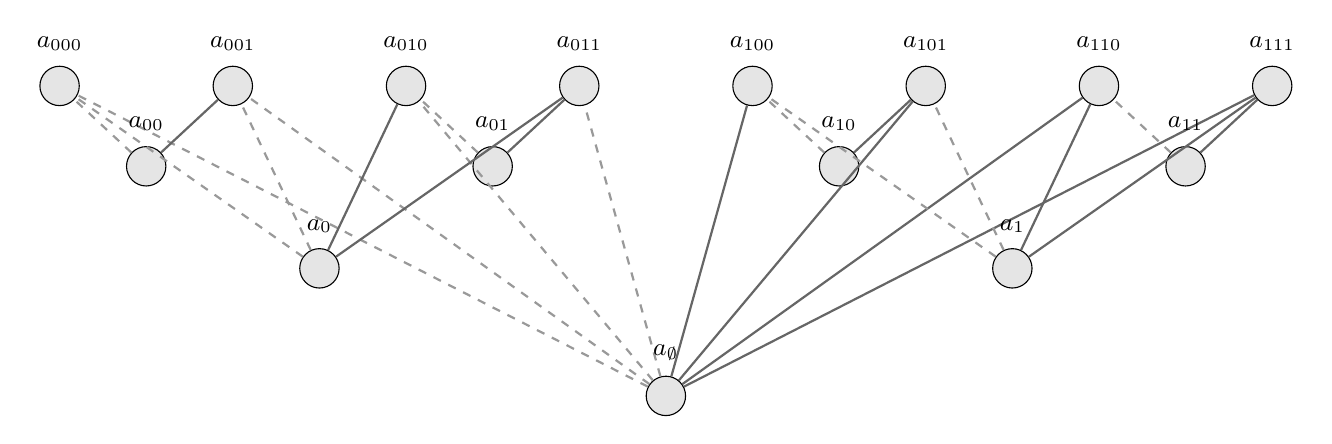
\begin{tikzpicture}[
        vertex/.style={circle, draw, fill=gray!20, minimum size=5mm, inner sep=1pt},
        label/.style={above=2pt, font=\small},
        solid edge/.style={draw, thick, black!60},
        dashed edge/.style={draw, dashed, thick, black!40},
    ]
	\node[vertex] (a_) at (8.8,0.0) {};
	\node[vertex] (a_0) at (4.4,1.62) {};
	\node[vertex] (a_1) at (13.200000000000001,1.62) {};
	\node[vertex] (a_00) at (2.2,2.9160000000000004) {};
	\node[vertex] (a_01) at (6.6000000000000005,2.9160000000000004) {};
	\node[vertex] (a_10) at (11.0,2.9160000000000004) {};
	\node[vertex] (a_11) at (15.400000000000002,2.9160000000000004) {};
	\node[vertex] (a_000) at (1.1,3.9366000000000008) {};
	\node[vertex] (a_001) at (3.3000000000000003,3.9366000000000008) {};
	\node[vertex] (a_010) at (5.5,3.9366000000000008) {};
	\node[vertex] (a_011) at (7.700000000000001,3.9366000000000008) {};
	\node[vertex] (a_100) at (9.9,3.9366000000000008) {};
	\node[vertex] (a_101) at (12.100000000000001,3.9366000000000008) {};
	\node[vertex] (a_110) at (14.3,3.9366000000000008) {};
	\node[vertex] (a_111) at (16.5,3.9366000000000008) {};
	\draw[dashed edge] (a_) -- (a_000);
	\draw[dashed edge] (a_) -- (a_001);
	\draw[dashed edge] (a_) -- (a_010);
	\draw[dashed edge] (a_) -- (a_011);
	\draw[solid edge] (a_) -- (a_100);
	\draw[solid edge] (a_) -- (a_101);
	\draw[solid edge] (a_) -- (a_110);
	\draw[solid edge] (a_) -- (a_111);
	\draw[dashed edge] (a_0) -- (a_000);
	\draw[dashed edge] (a_0) -- (a_001);
	\draw[solid edge] (a_0) -- (a_010);
	\draw[solid edge] (a_0) -- (a_011);
	\draw[dashed edge] (a_1) -- (a_100);
	\draw[dashed edge] (a_1) -- (a_101);
	\draw[solid edge] (a_1) -- (a_110);
	\draw[solid edge] (a_1) -- (a_111);
	\draw[dashed edge] (a_00) -- (a_000);
	\draw[solid edge] (a_00) -- (a_001);
	\draw[dashed edge] (a_01) -- (a_010);
	\draw[solid edge] (a_01) -- (a_011);
	\draw[dashed edge] (a_10) -- (a_100);
	\draw[solid edge] (a_10) -- (a_101);
	\draw[dashed edge] (a_11) -- (a_110);
	\draw[solid edge] (a_11) -- (a_111);
	\node[label] at (a_.north) {$a_{\emptyset}$};
	\node[label] at (a_0.north) {$a_{0}$};
	\node[label] at (a_1.north) {$a_{1}$};
	\node[label] at (a_00.north) {$a_{00}$};
	\node[label] at (a_01.north) {$a_{01}$};
	\node[label] at (a_10.north) {$a_{10}$};
	\node[label] at (a_11.north) {$a_{11}$};
	\node[label] at (a_000.north) {$a_{000}$};
	\node[label] at (a_001.north) {$a_{001}$};
	\node[label] at (a_010.north) {$a_{010}$};
	\node[label] at (a_011.north) {$a_{011}$};
	\node[label] at (a_100.north) {$a_{100}$};
	\node[label] at (a_101.north) {$a_{101}$};
	\node[label] at (a_110.north) {$a_{110}$};
	\node[label] at (a_111.north) {$a_{111}$};
    \end{tikzpicture}
    \caption{Example of a 3-tree. 
Notice that connections between disjoint sub-trees are not defined, and may be edges or non-edges in 
any combination.}
    \label{fig:k_tree}
\end{figure}
